\section{Sistemas de proyección}
\label{sec:cap2-sistemas-de-proyeccion}
Durante el siglo XVII, cartógrafos especializados, como Mercator, demostraron que no sólo el uso de
un sistema de proyección matemático y un ajustado sistema de coordenadas mejoraba la fiabilidad de
las medidas y la localización de las áreas de tierra, sino que el registro de fenómenos espaciales
a través de un modelo convenido de distribución de fenómenos naturales y asentamientos humanos era
de un valor incalculable para la navegación, para la búsqueda de rutas y en la estrategia militar
\citep{llopis2006sistemas}.

\subsection{Coordenadas geográficas}
Las coordenadas geográficas proveen un sistema de referencia que utilizan coordenadas angulares
(latitud y longitud) cuyo fin es el de determinar los ángulos laterales de la superficie terrestre.
La latitud es el ángulo que existe entre un punto cualquiera y el Ecuador, medida sobre el
meridiano que pasa por dicho punto. La longitud mide el ángulo a lo largo del ecuador desde
cualquier punto de la Tierra.

\begin{figure}
\centering
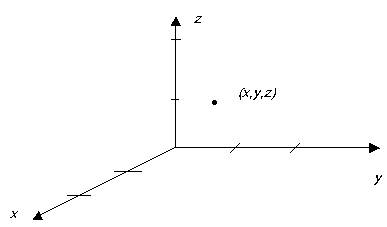
\includegraphics[width=0.5\textwidth]{capitulo-2/graphics/coordenadas-xyz.jpg}
\caption{\label{fig:sig-xyz} Represnetación de las coordenadas geográficas $(x,y,z)$.}
\end{figure}

Para la representación de objetos puntuales en una superficie, se utilizan las coordenadas X e Y
que caracterizan la planimetría y una coordenada Z que representa la altimertría del objeto en
cuestión.

\subsection{Proyecciones}
Se denomina proyecciones cartográficas o proyecciones geográficas al conjunto de métodos
utilizados para establecer una correspondencia matemática entre los puntos de la superficie curva
de la tierra y sus transformaciones en una superficie plana.

El problema principal a la hora de realizar una proyección es que no existe forma de representar
un una superficie plana toda la superficie curva, de la tierra, sin deformarla
\citep{llopis2006sistemas}. Teniendo en cuenta que la curvatura de la superficie terrestre es
proporcional al tamaño del área representada \citep{llopis2006sistemas}, si el área o región que se
desea representar es pequeña, entonces la deformación o distorsión resultante es despreciable, por
lo que puede ser modelada con coordenadas planas.

Con la aparición y difusión de los SIG, el conjunto de herramientas que ofrece se dio paso a
posibilidad de combinar información de diferentes mapas con diferentes proyecciones, esto ha
incrementado la relevancia de la cartografía más allá de la simple confección de mapas
\citep{llopis2006sistemas}.


\subsection{Elementos de representación cartográfica}
Para representar un objeto cualquiera o un fenómeno geográfico en un mapa es fundamental conocer
las características de este dato que contempla los tres aspectos siguientes: dimensiones, nivel de
medida y distribución. El análisis de las características de los elementos permite elegir la
simbología más adecuada para representar los fenómenos geográficos.

A cada entidad espacial se puede asociar diversas variables han desarrollado un amplio conjunto de
técnicas para cartografiar los hechos de la superficie terrestre.

\subsubsection{Dimensiones}
Por su extensión, los fenómenos que se representan en un mapa pueden clasificarse como puntuales,
lineales, poligonales o espacio-temporales.

\begin{itemize}
    \item Fenómenos puntuales : indican la presencia de entidades de un modo puntual. Pueden representarse
    utilizando diferentes símbolos o colores para una variable cualitativa, o diferentes tamaños para variables
    cuantitativas.

    \item Fenómenos lineales : simbolizan entidades, naturales o artificiales, de forma lineal conformadas a
    partir de la unión de varios puntos. Pueden utilizarse diferentes anchuras de linea, diferentes colores o
    diferentes tipos de linea para representar propiedades como la anchura de los ríos o categorías de vías de
    comunicación.

    \item Fenómenos Poligonales : La información puede ser bidimensional o tridimensional, que, por su tamaño,
    pueden ser representados como polígonos o porciones homogéneas del terreno en relación a una variable
    cualitativa. Pueden utilizarse diferentes colores o tramas para representar variables cualitativas o
    cuantitativas.

    \item Fenómenos espacio-temporales : La información depende del movimiento del fenómeno con respecto al paso
    del tiempo (migraciones de aves, expansión de una civilización,etc.).
\end{itemize}

\subsubsection{Nivel de medida}
Los elementos de la naturaleza se miden con el fin de clasificarlos y compararlos; lo que no
siempre implica una magnitud cuantitativa, ya que puede ser cualitativa u jerárquica. En orden
creciente de precisión tenemos:
\begin{itemize}
    \item Escala nominal : asigna una característica no numérica a un fenómeno, por lo que sólo se pueden hacer comparaciones de tipo cualitativo. Por ejemplo, un mapa de cuencas hidrográficas, un mapa de suelos. Este es el nivel más elemental de medida, pues no informa acerca de la cantidad o el orden.

    \item Escala ordinal : establece una cierta jerarquía no mensurable o no cuantificable entre los diferentes elementos. Por ejemplo, un mapa en el que aparecen núcleos de población, cuyos símbolos están jerarquizados según el número de habitantes sin especificar cantidad.

    \item Escala cuantitativa o de intervalo : La escala cuantitativa o de intervalo asigna una característica numérica a un fenómeno geográfico. Por ejemplo, en un mapa de temperaturas medias los intervalos son valores numéricos (expresados en grados Celsius o Fahrenheit). Es necesario emplear algún tipo de unidad convencional.
\end{itemize}

\subsubsection{Distribución}
La ocurrencia de un fenómeno sobre una superficie terrestre puede darse a lo largo y ancho de toda
ella, o de forma discontinua, dándose el fenómeno en alguna localización del territorio. Los
fenómenos en cuestión son :

\begin{itemize}
    \item Fenómenos continuos :  son los que tienen presencia en todos los puntos del territorio objeto de representación, aunque sólo se tengan medidas de algunos puntos significativos. Por ejemplo: la temperatura, altitud sobre en nivel del mar, niveles de contaminación atmosférica,densidad poblacional, etc.

    \item Fenómenos discretos : son los que tiene presencia en algunos puntos del territorio objeto de representación. Un ejemplo son los datos de población, dado que se localizan en determinadas áreas y no en todos los puntos del territorio. Algunos fenómenos discretos pueden transformarse en continuos mediante la aplicación de una relación. Por ejemplo, el número de habitantes de una provincia (fenómeno discreto) pasa a ser un fenómeno continuo cuando se habla de densidad de población: la relación se aplica dividiendo el número de habitantes por la superficie de la provincia en $km^2$
\end{itemize}
